% Template for a Thesis
%
% 3-tokenization.tex
%
% Tokenization

\chapter{Tokenization}\label{sec:tokenization}

\section{Introduction}

Tokenization is the first major step in language processing. The main idea is simplifying or compressing the input text into meaningful units, called tokens, creating a big vocabulary of tokens and shorter sequences, as illustrated in Figure 3.1.~\cite{manning2008introduction}

\begin{figure}[!ht]
    \centering
    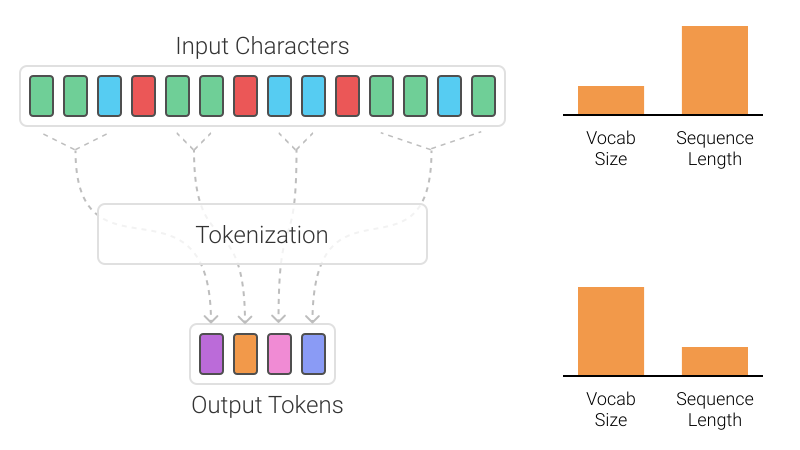
\includegraphics[width=14cm]{figures/tokenization.png}
    \caption{Tokenization of a sequence of text}
\end{figure}

\textbf{Tokens} in language are defined as units which have a semantic meaning, be it words, phrases, symbols or other elements. Here is an example of a simple way to tokenize text:

\begin{quote}
    Raw text: I ate a burger today, and it was good.\\
    Text after tokenization: ['I', 'ate', 'a', 'burger', 'today', 'and', 'it', 'was', 'good']
\end{quote}

In this example, the tokenization process is simple. First, locate the word boundaries and split words by whitespaces. Next, remove symbols and punctuation marks as both contain no definitive meaning. However, tokenization in real life is not always that easy: some punctuation marks are relevant to the meaning of the words around them.

\paragraph{How to deal with punctuation marks?}

Every language has its challenges. In ENglish for example, there are possessors such as \emph{aren't}, and contractions such as \emph{Sarah's} and \emph{O'Neill}. Because of this, it is imperative to know the language of the input text. \textit{Language identification} is the task of identifying the language of the input text. Methods ranging from the initial k-gram algorithms used in cryptography (Konnheim, 1981), to more modern n-gram methods (Dunning, 1994) are commonly used. Once the language is identified, we can follow the rules for each case and deal with punctuation marks appropriately.

\paragraph{Other types of tokens}

In the simple example above, tokens were words. Alternatively, tokens can be groups of words, characters or subwords (parts of a word). For example, take the word \emph{smarter}:

\begin{itemize}
    \item Sentence: the smarter computer
    \item Word tokens: the, smarter, computer
    \item Character tokens: t, h, e, s, m, a, r, t, e, r, c, o, m, p, u, t, e, r
    \item Subword tokens: the, smart, er, comput, er
    \item Subword tokens without word boundaries: the smart, er comput, er
\end{itemize}

The major question in the tokenization phase is: \textbf{what are the correct tokens to use?}. The following section explores these 4 types of tokenization methods and delves into the algorithms and code libraries available.

\section{Tokenization algorithm types}

The tokenization method depends heavily on the targeted application. This results in different applications requiring different tokenization algorithms. Nowadays, most deep learning architectures in NLP process raw text at the token level and as a first step, create embeddings for these tokens, which will be explained in more detail in the following section. In short, \textit{the type of tokenization depends on the type of embedding}. Advantages and drawbacks of several tokenization methods are further explained in the following sections.

\subsection{Word level tokenization}

Word level tokenization is the first established type of tokenization. It is the most basic and also the most common form of tokenization. It splits a piece of text into individual words based on word boundaries; usually a specific delimiter consisting mostly of whitespace ' ' or other punctuation signs.

Conceptually, splitting on whitespace can also split an element which should be regarded as a single token, for example New York. This is mostly the case with names, borrowed foreign phrases, and compounds that are sometimes written as multiple words. Tokenization without word boundaries aims to address that problem.~\ref{subsec:wordtokwowb} on page~\pageref{subsec:wordtokwowb}

\subsubsection{Word level algorithms}

The simplest way to obtain word level tokenization is by splitting the sentence on the desired delimeter; most commonly this is whitespace. The \pyth{sentence.split()} function in Python or a Regex command \pyth{re.findall("[\w']+", text)} achieves this in a simple way.

The \href{https://www.nltk.org/}{natural language toolkit (NLTK)} in Python provides a \href{https://www.nltk.org/api/nltk.tokenize.html}{tokenize package} which includes a \emph{word\_tokenize} function. The user can provide the language of the text, whereby if none is given, English is taken as default.

\begin{python}
from nltk.tokenize import word_tokenize
sentence = u'I spent $2 yesterday'
sentence_tokenized = word_tokenize(sentence, language='English')
>>> sentence_tokenized = ['I', 'spent', '$', '2', 'yesterday']
\end{python}

Comparatively, SpaCy offers a similar functionality. It is possible to load the language model for different languages and model size. In this case, the English language (en) and small model size (sm) was loaded.

\begin{python}
import spacy
sp = spacy.load('en_core_web_sm')
sentence = u'I spent $2 yesterday'
sentence_tokenized = sp(sentence)
>>> sentence_tokenized = ['I', 'spent', '$', '2', 'yesterday']
\end{python}

Other word level tokenization functions include Keras:

\begin{python}
from keras.preprocessing.text import text_to_word_sequence
sentence_tokenized = text_to_word_sequence(sentence)
\end{python}

And Gensim:

\begin{python}
from gensim.utils import tokenize
sentence_tokenized = list(tokenize(sentence))
\end{python}

Depending on the target application and framework, one might favor an algorithm over the other.

\paragraph{Word embeddings}\label{subsec:wordemb}

As stated before, the goal of tokenization is to split the text into units with meaning. Typically, each token is assigned an embedding vector. Word2vec (Mikolov et al., 2013~\cite{mikolov2013efficient}) is a way of transforming a word into a fixed-size vector representation, as shown in Figure 3.2.

\begin{figure}[!ht]
    \centering
    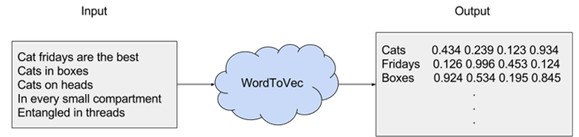
\includegraphics[width=14cm]{figures/word_emb.png}
    \caption{Representation of word embeddings}
\end{figure}

Apart from word2vec, there are other word embedding algorithms, namely \textit{GloVe} or \textit{fasttext}. When words are translated into a multi-dimensional (N) plane, each word can be compared relative to another. As such, words with similar context will appear closer to one another. Here is a simplified example to illustrate the concept of word embeddings.

\begin{itemize}
    \item Word: smart. Embedding: [2, 3, 1, 4]
    \item Word: intelligent. Embedding: [2, 3, 2, 3]
    \item Word: stupid. Embedding: [-2, -4, -1, -3]
\end{itemize}

In the example, the embeddings of \emph{smart} and \emph{intelligent} have a distance of 2, since the last two numbers in the vector differ by one respectively. If this was plotted in a four dimensional space, these words would be very close together. On the other hand, \emph{stupid} is almost the opposite of \emph{smart}. The distance in this case is much larger. In the plot, these words would sit roughly in opposite directions. Thus, with word embeddings, a sentence is transformed into a sequence of embedding vectors, which is very useful for NLP tasks.

\subsubsection{Word level tokenization drawbacks}

Word embeddings have some drawbacks. In many cases, a word can have more than one meaning: \emph{well}, for example, can be used in these two scenarios.

\begin{quote}
    I'm doing quite well.\\
    The well was full of water.
\end{quote}

In the first case, \textit{well} is an adverb and in the second it is a noun. \emph{well}'s embedding will probably be a mixture of the two, since word embeddings do not generalize to \textbf{homonyms}. Consequently, the true meaning of both words cannot be represented.

Another drawback is that word embeddings are not well equipped to deal with \textbf{out of vocabulary (oov) words}. Word embeddings are created based on limited vocabulary size known to the system. If a foreign or misspelled word is detected, it will be given a universal unknown <UNK> embedding, that will be the same for all unknown words. Therefore, all unknown words in NLP will be treated similarly as if they have the same meaning. The information within these words is lost due to the mapping from OOV to UNK.

Another issue with word tokens is related to the \textbf{vocabulary size}. Generally, pre-trained models are trained on a large volume of the text corpus. As such, if the vocabulary is built with all the unique words in such a large corpus, it creates a huge vocabulary. This opens the door to \emph{character tokenization}, since in this case the vocabulary depends on the number of characters, which is significantly lower than the number of all different words.

These problems are not to be mistaken with tokenization problems, tokenization is merely a way to an end. In most cases however, they are used to create embeddings. And if embeddings from word tokens have drawbacks, the tokenization method is changed in order to create different tokens, in order to create other types of embeddings.
    
\subsection{Character level tokenization}

In this type of tokenization, instead of splitting a text into words, the splitting is done into characters, whereby \emph{smarter} becomes \emph{s-m-a-r-t-e-r} for instance. \href{https://github.com/karpathy/char-rnn}{Karpathy, 2015} was the first to introduce a character level language model.

OOV words, misspellings or rare words are handled better, since they are broken down into characters and these characters are usually known in the vocabulary. In addition, the size of the vocabulary is significantly lower, namely 26 in the simple case where only the English characters are considered, though one might as well include all ASCII characters. Zhang et al. (2015)~\cite{zhang2015text}, who introduced the character CNN, consider all the alphanumeric character, in addition to puctuation marks and some special symbols.

Character level models are unrestricted in their vocabulary and see the input "as-is". Since the vocabulary is much lower, the model's performance is much better than in the word tokens case. Tokenizing sequences at the character level has shown some impressive results.

Radfor et al. (2017)~\cite{radford2017learning} from OpenAI showed that character level models can capture the semantic properties of text. Kalchbrenner et al.(2016)~\cite{kalchbrenner2016neural} from Deepmind and Leet et al. (2017)~\cite{lee-etal-2017-fully} both demonstrated translation at the character level. These are particularly compelling results as the task of translation captures the semantic understanding of the underlying text.

\subsubsection{Character level algorithms}

The previous libraries explored in the case of word tokenization (native python libraries, nltk, spacy, keras) have their own version for character level tokenization.

\subsubsection{Character level tokenization drawbacks}

When tokenizing a text at the character level, the sequences are longer, which takes longer to compute since the neural network needs to have significantly more parameters to allow the model to perform the conceptual grouping internally, instead of being handed the groups from the beginning.

It becomes challenging to learn the relationship between the characters to form meaningful words and, given that there is no semantic information among characters, characters are semantically void. This makes it complicated to generate character embeddings.

Sometimes the NLP task does not need processing at the character level, such as when doing a sequence tagging task or name entity recognition, the character level model will output characters, which requires post processing.

As an in-betweener between word and character tokenization, subword tokenization produces subword units, smaller than words but bigger than just characters.

\subsection{Subword level tokenization}

Subword tokenization is the task of splitting the text into subwords or n-gram characters. For example, words like \emph{lower} can be segmented as \emph{low-er}, \emph{smartest} as \emph{smart-est}, and so on. In the event of an OOV word such as \emph{eorner}, this tokenizer will divide it into \emph{eorn-er} and effectivey obtain some semantic information. Very common subwords such as \emph{ing}, \emph{ion}, usually with a morphological sense, are learnt through repetition. The word \emph{unfriendly} would be split into \emph{un-friend-ly}.

\begin{figure}[!ht]
    \centering
    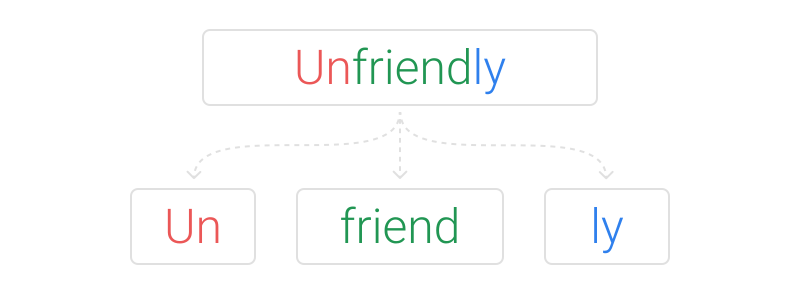
\includegraphics[width=10cm]{figures/subword.png}
    \caption{Representation of the word 'unfriendly' in subword units}
\end{figure}

At the time of writing (2020), the most powerful deep learning architectures are based on Transformers (Vaswani et al., 2017~\cite{vaswani2017attention}), and these rely on subword tokenization algorithms to prepare the vocabulary.

\paragraph{Subword level algorithms}

Since Transformers are a relatively new architecture in 2020, subword tokenization is an active area of research. Nowadays four algorithms stand out: byte-pair encoding (BPE), unigram LM, WordPiece and SentencePiece.

Since BPE is the basis of the thesis, it will be explained in depth in the following section. A simple explanation of BPE and the rest of the algorithms follow below.

Huggingface, an open source NLP company, released Transformers and Tokenizers (Wolf et al., 2019~\cite{wolf2019huggingfaces}), two popular NLP framework which include \href{https://github.com/huggingface/tokenizers/tree/74d812d40180032d2dbb6ca59e2e10f0257ef46b/bindings/python/tokenizers/implementations}{several subword tokenizers} such as \emph{ByteLevelBPETokenizer}, \emph{CharBPETokenizer}, \emph{SentencePieceBPETokenizer} and \emph{BertWordPieceTokenizer}. The first refer to the first subword level algorithm, BPE, in addition to WordPiece and SentencePiece.

\subsubsection{BPE}\label{subsubsec:bpe}

BPE (Sennrich et al., 2016~\cite{sennrich2015neural}) merges the most frequently occurring character or character sequences iteratively. This is roughly how the algorithm works:

\begin{enumerate}
    \item Get a large enough corpus.
    \item Define a desired subword vocabulary size.
    \item Split word to sequence of characters and append a special token showing the beginning-of-word or end-of-word affix/suffix respectively.
    \item Calculate pairs of sequences in the text and their frequencies. For example, ('t', 'h') has frequency X, ('h', 'e') has frequency Y.
    \item Generate a new subword according to the pairs of sequences that occurs most frequently. For example, if ('t', 'h') has the highest frequency in the set of pairs, the new subword unit would become 'th'.
    \item Repeat from step 3 until reaching subword vocabulary size (defined in step 2) or the next highest frequency pair is 1. Following the example, ('t', 'h') would be replaced by 'th' in the corpus, the pairs calculated again, the most frequent pair obtained again, and merged again.
\end{enumerate}

BPE is based on a greedy and deterministic symbol replacement, and ca not provide multiple segmentations.

\subsubsection{Unigram LM}\label{subsubsec:unigramlm}

Unigram language modeling (Kudo, 2018~\cite{kudo-2018-subword}) is based on the assumption that all subword occurrences are independent and therefore subword sequences are produced by the product of subword occurrence probabilities. These are the steps of the algorithm:

\begin{enumerate}
    \item Get a large enough corpus.
    \item Define a desired subword vocabulary size.
    \item Optimize the probability of word occurrence by giving a word sequence.
    \item Compute the loss of each subword.
    \item Sort the symbol by loss and keep top X \% of word (X=80\% for example). To avoid oov instances, character level is recommended to be included as a subset of subwords.
    \item Repeat step 3–5 until reaching the subword vocabulary size (defined in step 2) or there are no changes (step 5).
\end{enumerate}

Kudo argues that the unigram LM model is more flexible than BPE because it is based on a probabilistic LM and can output multiple segmentations with their probabilities.

\subsubsection{WordPiece}\label{subsubsec:wordpiece}

WordPiece (Schuster and Nakajima, 2012~\cite{schuster2012japanese}) was initially used to solve Japanese and Korean voice problem. It is similar to BPE in many ways, except that it forms a new subword based on likelihood, not on the next highest frequency pair. These are the steps of the algorithm:

\begin{enumerate}
    \item Get a large enough corpus.
    \item Define a desired subword vocabulary size.
    \item Split word to sequence of characters.
    \item Initialize the vocabulary with all the characters in the text.
    \item Build a language model based on the vocabulary.
    \item Generate a new subword unit by combining two units out of the current vocabulary to increment the vocabulary by one. Choose the new subword unit out of all the possibilities that increases the likelihood on the training data the most when added to the model.
    \item Repeat step 5 until reaching subword vocabulary size (defined in step 2) or the likelihood increase falls below a certain threshold.
\end{enumerate}

WordPiece and BPE only differ in step 6, since BPE merges the token combination that has the maximum frequency. This frequency stems from the combination of the tokens and not previous individual tokens. In WordPiece, the frequency of the two tokens are separately taken into account. If there are 2 tokens A and B, the score of this combination will be the following:

\begin{quote}
    Score(A,B) = Frequency(A,B) / Frequency(A) * Frequency(B)
\end{quote}

The token pair with the highest score will be selected. It might be the case that \textit{Frequency('so', 'on')} is very high but their individual frequencies are also high. Hence with the WordPiece algorithm, 'soon' will not be merged as the overall score is low. In another example, \textit{Frequency('Jag','gery')} might be low but if their individual frequencies are also low, 'Jag' and 'gery' might be joined to form 'Jaggery'.

BERT (Devlin et al., 2018~\cite{devlin2018bert}) uses WordPiece as its tokenization method, yet the precise tokenization algorithm and/or code has not been made public. This example shows the tokenization step and how it handles OOV words.

\begin{quote}
    original tokens = ["John", "Johanson", "'s",  "house"]
    bert tokens = ["[CLS]", "john", "johan", "\#\#son", "'", "s", "house", "[SEP]"]
\end{quote}

\subsubsection{SentencePiece}

SentencePiece (Kudo et al. 2018~\cite{kudo2018sentencepiece}) is a subword tokenization type that has an \href{https://github.com/google/sentencepiece}{extensive Github repository} with freely available code.

As the repository states, it is an unsupervised text tokenizer and detokenizer where the vocabulary size is predetermined prior to the neural model training. It implements subword units (e.g., BPE~\ref{subsubsec:bpe}) and unigram LM~\ref{subsubsec:unigramlm}) with the extension of direct training from raw sentences. It does not depend on language-specific pre or post-processing.

While conceptually similar to BPE, it does not use the greedy encoding strategy, thus achieving higher quality tokenization while reducing error induced by location-dependent factors as seen in BPE. SentencePiece sees ambiguity in character grouping as a source of regularization for downstream models during training, and uses a simple language model to evaluate the most likely character groupings instead of greedily picking the longest recognized strings like BPE does.

Approaching ambiguity in text as a regularization parameter for downstream models results in higher tokenization quality but adversely reduces the performance of the pipeline, at times making it the slowest part or bottleneck of an NLP system. While the assumption of ambiguity in tokenization seems natural, it appears the performance trade-off is not worth it, as Google itself opted not to use this strategy in their BERT language model.~\ref{subsubsec:wordpiece}

\begin{figure}[!ht]
    \centering
    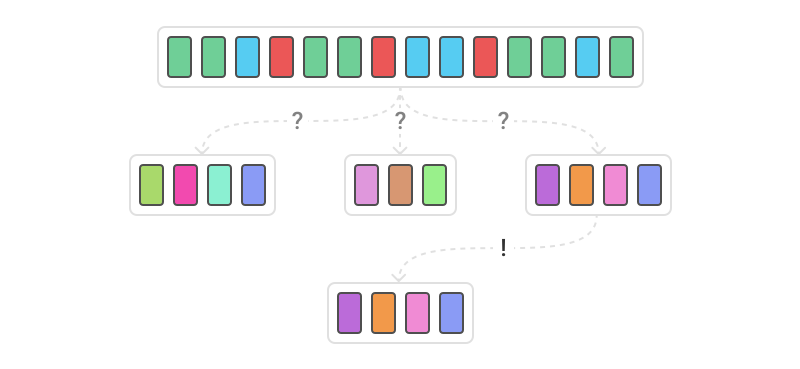
\includegraphics[width=14cm]{figures/sentencepiece.png}
    \caption{Representation of the SentencePiece tokenization in a sequence of text}
\end{figure}

The number of unique tokens in SentencePiece is predetermined, the segmentation model is trained such that the final vocabulary size is fixed, e.g., 8k, 16k, or 32k. This is different from BPE (Sennrich et al., 2015~\cite{sennrich2015neural}) which uses the number of merge operations instead. The number of merge operations is a BPE-specific parameter and not applicable to other segmentation algorithms, including unigram, word and character level algorithms.

\subsection{Tokenization without word boundaries}\label{subsec:wordtokwowb}

Another type of tokenization, beyond word, character or subword, is tokenization without word boundaries. The three types of tokenization explored until now cannot create units among words, that is, they consider words separatedly.

When dealing with languages that do not include space tokenization, such as several Asian languages, an individual symbol can resemble a syllable rather than a word or letter. Most words are short (the most common length is 2 characters), and given the lack of standardization of word breaks in the writing system or lack of punctuation in certain languages, it is not always clear where word boundaries should be placed. As an example, in English:

\begin{quote}
    Input sentence: the smarter computer\\
    Subword tokens without word boundaries: the smart, er comput, er
\end{quote}

An approach to handle this has been to abandon word-based indexing, and do all indexing from just short subsequences of characters (character n-grams), regardless of whether particular sequences cross word boundaries or not. Hence, at times, each character used is taken as a token in Chinese tokenization.

\section{BPE}

Byte Pair Encoding (BPE) (Sennrich et al., 2015~\cite{sennrich2015neural}), is a widely used tokenization method among Transformer-based models. The code is open source and there is an \href{https://github.com/rsennrich/subword-nmt}{active repository} on Github. It merges the most frequently occurring character or character sequences iteratively.

\begin{figure}[!ht]
    \centering
    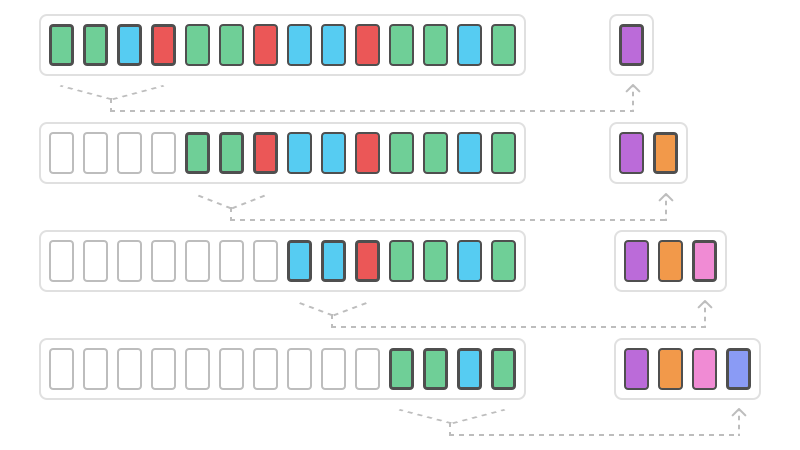
\includegraphics[width=14cm]{figures/bpe.png}
    \caption{Representation of the BPE tokenization in a sequence of text}
\end{figure}

BPE enables the encoding of rare or OOV words with appropriate subword tokenization without introducing any 'unknown' tokens. One of the performance aspects in tokenization is the length of output sequences. Here, BPE is superior as it produces shorter sequences compared to character tokenization.

\subsection{Minimal algorithm to learn BPE segmentations}

Subsection ~\ref{subsubsec:bpe} showed a simple algorithm to build subword units. In this section it will be explained in depth with an example. These are the steps of the algorithm:

\begin{enumerate}
    \item Get a large enough corpus.
    \item Define a desired subword vocabulary size.
    \item Split word to sequence of characters and append a special token showing the beginning-of-word or end-of-word affix/suffix respectively.
    \item Calculate pairs of sequences in the text and their frequencies.
    \item Generate a new subword according to the pairs of sequences that occurs most frequently, and save it to the vocabulary.
    \item Merge the most frequent pair in corpus.
    \item Repeat from step 4 until reaching subword vocabulary size (defined in step 2) or the next highest frequency pair is 1.
\end{enumerate}

Considering a simple corpus with a single line, and a desired subword vocabulary size of 10. The character \emph{'\_'} marks the beginning of each word. The following code shows the steps 1-3.

\begin{python}
def read_corpus(corpus):
    tokens = [("_" + " ".join(token)) for token in corpus]
    return tokens

corpus = ['this is this.']
vocab_size = 10
tokens = read_corpus(corpus)
>>> tokens = ['_t h i s _i s _t h i s .']
\end{python}

Now we can calculate the pairs of characters and their frequencies, as well as the most popular pair. These are the steps 4-5 in the algorithm above.

\begin{python}
from collections import Counter

def get_stats(tokens):
    pairs = Counter()
    for sent in tokens:
        for word in sent[1:].split(' _'):
            symbols = ('_' + word).split()
            for j in range(len(symbols) - 1):
                pairs[symbols[j], symbols[j+1]] += 1
    return pairs

pairs = get_stats(tokens)
>>> pairs = Counter({('_t', 'h'): 2, ('h', 'i'): 2, ('i', 's'): 2, 
                    ('_i', 's'): 1, ('i', 's,'): 1, ('_', 'i'): 1, 
                    ('_i', 't'): 1, ('t', '?'): 1})

most_frequent_pair = pairs.most_common(1)[0][0]
>>> most_frequent_pair = ('_t', 'h')

vocab = []
vocab.append(most_frequent_pair)
\end{python}

There we can see each bigram and its frequency. For example, ('\_t', 'h') occurs twice in the corpus, and it is taken as the most frequently occurring bigram, which we can save into the merge\_list. Now it is the time to merge this pair in the corpus as stated in step 6.

\begin{python}
import re

def merge_pair_in_corpus(tokens, pair):
    # convert list of sentences into one big string
    # in order to do the substitution once
    tokens = '\n'.join(tokens)

    # regex to capture the pair
    p = re.compile(r'(?<!\S)' + re.escape(' '.join(pair)) + r'(?!\S)')

    # substitute the unmerged pair by the merged pair
    tokens = p.sub(''.join(pair), tokens)

    tokens = tokens.split('\n')
    return tokens

tokens = merge_pair_in_corpus(tokens, most_frequent_pair)
>>> tokens = ['_th i s _i s _th i s .']
\end{python}

The subword unit '\_th' has been created, saved in the vocabulary and merged in the corpus. The last step is iterating until the subword vocabulary size has been reached or until there are no pairs with bigger than 1. At each step, the object \emph{pairs} is computed again since there might be new pairs such as ('\_th', 'i') in this example. The whole minimal code would look like this:

\begin{python}
corpus = ['this is this.']
vocab_size = 10
vocab = []

tokens = read_corpus(corpus)

for _ in range(vocab_size):

    pairs = get_stats(tokens)

    # frequency of the most common pair is 1, break loop
    if pairs.most_common(1)[0][1] == 1:
        break

    most_frequent_pair = pairs.most_common(1)[0][0]
    vocab.append(most_frequent_pair)
    tokens = merge_pair_in_corpus(tokens, most_frequent_pair)

>>> tokens = ['_this _i s _this .']
\end{python}

In each step of the iteration, the \emph{get\_stats} function iterates all the characters in the corpus, so the complexity is O(len(corpus) * length of sentence), for an average sentence length. Obtaining the most frequent pair takes constant time, since the object \emph{pairs} is a Counter object and includes a function to retrieve the most frequent item. At the step of \emph{merge\_pair\_in\_corpus}, the corpus is iterated in its entirety again, with a complexity of O(len(corpus) * len(sent)). Therefore, the algorithm has a complexity of O(num\_merges * len(corpus) * len(sent)). Iterating num\_merges amount of times cannot be avoided, but operating through all the characters in the corpus is computationally very expensive. One of the contributions of this thesis is an optimization of this algorithm, as will be shown in the following chapters.

\subsection{Applying BPE to OOV words}

In the event of an OOV word, such as 'these', which the corpus used in the previous example does not know, the BPE algorithm can create some subword units from the corpus used before.

\begin{enumerate}
    \item Split the OOV word into characters after inserting '\_' in the beginning.
    \item Compute the pair of character or character sequences in the OOV word.
    \item Select the pairs present in the learned operations.
    \item Merge the most frequent pair.
    \item Repeat steps 2-4 until merging is possible.
\end{enumerate}

And this is the code in Python for such an algorithm:

\begin{python}
oov = 'these'
oov = ['_' + ' '.join(list(oov))]

i = 0
while True:
    pairs = get_stats(oov)
    # find the pairs available in the vocab learnt before
    idx = [vocab.index(i) for i in pairs if i in vocab]

    if len(idx) == 0:
        print("BPE completed")
        break

    # choose the most frequent pair which appears in the OOV word
    best = merges[min(idx)]

    # merge the best pair
    oov = merge_vocab(best, oov)

>>> oov = '_th e s e'
\end{python}

'\_th' is the only known merge in the vocabulary, the rest of the characters ('e', 's', 'e') are unknown to the vocabulary so it does not know how to create any subword units.

\subsection{BPE dropout}

BPE dropout (Provilkov et al., 2019~\cite{provilkov2019bpedropout}) changes the BPE algorithm by stochastically corrupting the segmentation procedure of BPE, producing multiple segmentations within the same fixed BPE framework.

It exploits the innate ability of BPE to be stochastic: the merge table remains the same, but when applying it to the corpus, at each merge step some merges are randomly dropped with probability p, hence the name of BPE dropout. In the paper p=0.1 is used during training and p=0 during inference. For the Chinese and Japanese languages, p=0.6 is used in order to match the increase in length of segmented sentences as other languages.

It's hypothesized in the paper that exposing a model to different segmentations might result in better understanding of the whole words as well as their subword units. The performance improvement with respect to normal BPE is consistent no matter the vocabulary size, but it is shown that the impact from using BPE-Dropout vanishes when a corpora size gets bigger. These results are replicated and confirmed in later chapters.

Sentences segmented with BPE-Dropout are longer. There is a danger that models trained with BPE-Dropout might use more fine-grained segmentation during inference and hence slow down the process.

\subsection{BPE drawbacks}

Kudo (2018)~\cite{kudo-2018-subword} showed that BPE is a \textbf{greedy algorithm} that keeps the most frequent words intact, while splitting the rare ones into multiple tokens. BPE splits words into unique sequences, meaning that for each word, a model observes \textbf{only one segmentation}, meaning that if there is a segmentation error, all the following steps are erroneous. Additionally, subwords into which rare words are segmented end up poorly understood.

Although the problem of unique segmentation can be improved with the BPE Dropout method, it is still susceptible to the common problems of BPE, namely, the greediness of the algorithm and fragility regarding segmentation errors, problems which are explored in the following chapters.
